\documentclass[11pt]{article}
\usepackage[margin=1in]{geometry}
\usepackage{booktabs,amsmath,amssymb,amsthm,graphicx,url,array,xcolor}
\usepackage[colorlinks=true,linkcolor=blue!50!black,citecolor=blue!50!black,urlcolor=blue!50!black]{hyperref}
% AUTO-GENERATED by make_numbers.py. Do not edit.
\newcommand{\OneMismatchShared}{0/900} % H1_H3/*/O1_mismatch_rate_shared
\newcommand{\OneMismatchNaive}{0/900} % H1_H3/*/O1_mismatch_rate_naive
\newcommand{\OneMismatchKeyed}{0/900} % H1_H3/*/O1_mismatch_rate_keyed
\newcommand{\RhoTwoShared}{0.80} % H1_H3/S2/rho/shared
\newcommand{\RhoTwoSharedCI}{[0.66, 0.89]} % H1_H3/S2/rho/shared/ci
\newcommand{\RhoTwoNaive}{0.63} % H1_H3/S2/rho/naive
\newcommand{\RhoTwoNaiveCI}{[0.28, 0.82]} % H1_H3/S2/rho/naive/ci
\newcommand{\RhoTwoKeyed}{0.86} % H1_H3/S2/rho/keyed
\newcommand{\RhoTwoKeyedCI}{[0.65, 0.95]} % H1_H3/S2/rho/keyed/ci
\newcommand{\DeltaRhoTwo}{0.06} % H1_H3/S2/delta_rho_keyed_minus_shared
\newcommand{\DeltaRhoTwoCI}{[-0.16, 0.23]} % H1_H3/S2/delta_rho_keyed_minus_shared/ci
\newcommand{\DeltaRhoNaiveTwo}{0.23} % H1_H3/S2/delta_rho_keyed_minus_naive
\newcommand{\DeltaRhoNaiveTwoCI}{[-0.04, 0.58]} % H1_H3/S2/delta_rho_keyed_minus_naive/ci
\newcommand{\VRFTwo}{1.24} % H1_H3/S2/VRF_shared_over_keyed
\newcommand{\VRFTwoCI}{[0.57, 2.89]} % H1_H3/S2/VRF_shared_over_keyed/ci
\newcommand{\WidthRatioTwo}{0.88} % H1_H3/S2/H3_width_ratio_keyed_over_shared
\newcommand{\HOneVerdictTwo}{not supported} % H1_H3/S2/H1_confirmed
\newcommand{\HThreeVerdictTwo}{not confirmed} % H1_H3/S2/H3_confirmed
\newcommand{\MeanDTwoShared}{-0.040} % H1_H3/S2/H3_mean_d_shared/mean
\newcommand{\MeanDTwoSharedCI}{[-0.064, -0.017]} % H1_H3/S2/H3_mean_d_shared/ci
\newcommand{\PValTwoShared}{0.0008} % H1_H3/S2/H3_mean_d_shared/signflip_p
\newcommand{\MeanDTwoNaive}{-0.015} % H1_H3/S2/H3_mean_d_naive/mean
\newcommand{\MeanDTwoNaiveCI}{[-0.041, 0.010]} % H1_H3/S2/H3_mean_d_naive/ci
\newcommand{\PValTwoNaive}{0.2521} % H1_H3/S2/H3_mean_d_naive/signflip_p
\newcommand{\MeanDTwoKeyed}{-0.008} % H1_H3/S2/H3_mean_d_keyed/mean
\newcommand{\MeanDTwoKeyedCI}{[-0.028, 0.013]} % H1_H3/S2/H3_mean_d_keyed/ci
\newcommand{\PValTwoKeyed}{0.4535} % H1_H3/S2/H3_mean_d_keyed/signflip_p
\newcommand{\PropCDiffTwo}{0.016} % H1_H3/S2/PropC_FIFO_mean_M
\newcommand{\PropCSETwo}{0.028} % H1_H3/S2/PropC_FIFO_mean_M
\newcommand{\PropCOKTwo}{yes} % H1_H3/S2/PropC_FIFO_mean_M
\newcommand{\RhoFourShared}{0.66} % H1_H3/S4/rho/shared
\newcommand{\RhoFourSharedCI}{[0.48, 0.82]} % H1_H3/S4/rho/shared/ci
\newcommand{\RhoFourNaive}{0.75} % H1_H3/S4/rho/naive
\newcommand{\RhoFourNaiveCI}{[0.64, 0.84]} % H1_H3/S4/rho/naive/ci
\newcommand{\RhoFourKeyed}{0.69} % H1_H3/S4/rho/keyed
\newcommand{\RhoFourKeyedCI}{[0.56, 0.80]} % H1_H3/S4/rho/keyed/ci
\newcommand{\DeltaRhoFour}{0.03} % H1_H3/S4/delta_rho_keyed_minus_shared
\newcommand{\DeltaRhoFourCI}{[-0.18, 0.24]} % H1_H3/S4/delta_rho_keyed_minus_shared/ci
\newcommand{\DeltaRhoNaiveFour}{-0.05} % H1_H3/S4/delta_rho_keyed_minus_naive
\newcommand{\DeltaRhoNaiveFourCI}{[-0.22, 0.09]} % H1_H3/S4/delta_rho_keyed_minus_naive/ci
\newcommand{\VRFFour}{0.79} % H1_H3/S4/VRF_shared_over_keyed
\newcommand{\VRFFourCI}{[0.37, 1.58]} % H1_H3/S4/VRF_shared_over_keyed/ci
\newcommand{\WidthRatioFour}{1.14} % H1_H3/S4/H3_width_ratio_keyed_over_shared
\newcommand{\HOneVerdictFour}{not supported} % H1_H3/S4/H1_confirmed
\newcommand{\HThreeVerdictFour}{not confirmed} % H1_H3/S4/H3_confirmed
\newcommand{\MeanDFourShared}{-0.026} % H1_H3/S4/H3_mean_d_shared/mean
\newcommand{\MeanDFourSharedCI}{[-0.051, 0.002]} % H1_H3/S4/H3_mean_d_shared/ci
\newcommand{\PValFourShared}{0.0645} % H1_H3/S4/H3_mean_d_shared/signflip_p
\newcommand{\MeanDFourNaive}{-0.034} % H1_H3/S4/H3_mean_d_naive/mean
\newcommand{\MeanDFourNaiveCI}{[-0.058, -0.010]} % H1_H3/S4/H3_mean_d_naive/ci
\newcommand{\PValFourNaive}{0.0076} % H1_H3/S4/H3_mean_d_naive/signflip_p
\newcommand{\MeanDFourKeyed}{-0.041} % H1_H3/S4/H3_mean_d_keyed/mean
\newcommand{\MeanDFourKeyedCI}{[-0.072, -0.012]} % H1_H3/S4/H3_mean_d_keyed/ci
\newcommand{\PValFourKeyed}{0.0083} % H1_H3/S4/H3_mean_d_keyed/signflip_p
\newcommand{\PropCDiffFour}{0.007} % H1_H3/S4/PropC_FIFO_mean_M
\newcommand{\PropCSEFour}{0.027} % H1_H3/S4/PropC_FIFO_mean_M
\newcommand{\PropCOKFour}{yes} % H1_H3/S4/PropC_FIFO_mean_M
\newcommand{\RhoEightShared}{0.73} % H1_H3/S8/rho/shared
\newcommand{\RhoEightSharedCI}{[0.58, 0.85]} % H1_H3/S8/rho/shared/ci
\newcommand{\RhoEightNaive}{0.65} % H1_H3/S8/rho/naive
\newcommand{\RhoEightNaiveCI}{[0.49, 0.79]} % H1_H3/S8/rho/naive/ci
\newcommand{\RhoEightKeyed}{0.86} % H1_H3/S8/rho/keyed
\newcommand{\RhoEightKeyedCI}{[0.76, 0.92]} % H1_H3/S8/rho/keyed/ci
\newcommand{\DeltaRhoEight}{0.13} % H1_H3/S8/delta_rho_keyed_minus_shared
\newcommand{\DeltaRhoEightCI}{[-0.02, 0.30]} % H1_H3/S8/delta_rho_keyed_minus_shared/ci
\newcommand{\DeltaRhoNaiveEight}{0.21} % H1_H3/S8/delta_rho_keyed_minus_naive
\newcommand{\DeltaRhoNaiveEightCI}{[0.05, 0.37]} % H1_H3/S8/delta_rho_keyed_minus_naive/ci
\newcommand{\VRFEight}{1.37} % H1_H3/S8/VRF_shared_over_keyed
\newcommand{\VRFEightCI}{[0.75, 2.58]} % H1_H3/S8/VRF_shared_over_keyed/ci
\newcommand{\WidthRatioEight}{0.85} % H1_H3/S8/H3_width_ratio_keyed_over_shared
\newcommand{\HOneVerdictEight}{not supported} % H1_H3/S8/H1_confirmed
\newcommand{\HThreeVerdictEight}{not confirmed} % H1_H3/S8/H3_confirmed
\newcommand{\MeanDEightShared}{-0.026} % H1_H3/S8/H3_mean_d_shared/mean
\newcommand{\MeanDEightSharedCI}{[-0.058, 0.005]} % H1_H3/S8/H3_mean_d_shared/ci
\newcommand{\PValEightShared}{0.1128} % H1_H3/S8/H3_mean_d_shared/signflip_p
\newcommand{\MeanDEightNaive}{-0.035} % H1_H3/S8/H3_mean_d_naive/mean
\newcommand{\MeanDEightNaiveCI}{[-0.065, -0.004]} % H1_H3/S8/H3_mean_d_naive/ci
\newcommand{\PValEightNaive}{0.0290} % H1_H3/S8/H3_mean_d_naive/signflip_p
\newcommand{\MeanDEightKeyed}{-0.033} % H1_H3/S8/H3_mean_d_keyed/mean
\newcommand{\MeanDEightKeyedCI}{[-0.060, -0.006]} % H1_H3/S8/H3_mean_d_keyed/ci
\newcommand{\PValEightKeyed}{0.0177} % H1_H3/S8/H3_mean_d_keyed/signflip_p
\newcommand{\PropCDiffEight}{0.018} % H1_H3/S8/PropC_FIFO_mean_M
\newcommand{\PropCSEEight}{0.033} % H1_H3/S8/PropC_FIFO_mean_M
\newcommand{\PropCOKEight}{yes} % H1_H3/S8/PropC_FIFO_mean_M
\newcommand{\CostShared}{3.13} % H1_H3/S2/cost_wall_ms/shared/median_ms
\newcommand{\CostNaive}{4.18} % H1_H3/S2/cost_wall_ms/naive/median_ms
\newcommand{\CostKeyed}{7.44} % H1_H3/S2/cost_wall_ms/keyed/median_ms
\newcommand{\CostRatioKeyed}{2.38} % H1_H3/S2/cost_wall_ms keyed/shared
\newcommand{\UndelFracFIFO}{1.2\%} % H2/S2/FIFO/undelivered_fraction
\newcommand{\UndelFracFIFOCI}{[1.0\%, 1.3\%]} % H2/S2/FIFO/undelivered_fraction/ci
\newcommand{\UnderUFIFO}{-0.4\%} % H2/S2/FIFO/understatement_U
\newcommand{\UnderUFIFOCI}{[-0.5\%, -0.3\%]} % H2/S2/FIFO/understatement_U/ci
\newcommand{\UndelFracFullSASP}{1.2\%} % H2/S2/FullSASP/undelivered_fraction
\newcommand{\UndelFracFullSASPCI}{[1.0\%, 1.4\%]} % H2/S2/FullSASP/undelivered_fraction/ci
\newcommand{\UnderUFullSASP}{-0.2\%} % H2/S2/FullSASP/understatement_U
\newcommand{\UnderUFullSASPCI}{[-0.4\%, -0.1\%]} % H2/S2/FullSASP/understatement_U/ci
\newcommand{\UndelFracMeanOnly}{1.2\%} % H2/S2/MeanOnly/undelivered_fraction
\newcommand{\UndelFracMeanOnlyCI}{[1.0\%, 1.4\%]} % H2/S2/MeanOnly/undelivered_fraction/ci
\newcommand{\UnderUMeanOnly}{-0.3\%} % H2/S2/MeanOnly/understatement_U
\newcommand{\UnderUMeanOnlyCI}{[-0.4\%, -0.1\%]} % H2/S2/MeanOnly/understatement_U/ci
\newcommand{\LateDiscards}{0.00} % H2/S2/*/late_discards_per_run (max)
\newcommand{\RetryDrops}{0.00} % H2/S2/*/dropped_after_retry_per_run (max)
\newcommand{\GenPerRun}{238} % H2/S2/FIFO/generated_per_run
\newcommand{\DrainValid}{passed} % H2/drain_control/validity_check_passed
\newcommand{\DrainRows}{300} % H2/drain_control/fer0_rows
\newcommand{\DrainUndelFerOne}{0.00} % H2/drain_control/fer001_undelivered_per_run (max)
\newcommand{\RankFlip}{6\%} % H2/exploratory_ranking_flip_fraction_S2
\newcommand{\UndelThreshold}{2\%} % preregistration H2 threshold (constant)
\newcommand{\HTwoVerdict}{not material} % H2/*/all_arms_material
\newcommand{\HFourRatioFIFO}{54\%} % H4/FIFO/ratio
\newcommand{\HFourRatioFIFOCI}{[37\%, 75\%]} % H4/FIFO/ratio_ci
\newcommand{\HFourWithFIFO}{0.0049} % H4/FIFO/mean_S1_with
\newcommand{\HFourWithoutFIFO}{0.0057} % H4/FIFO/mean_S1_without
\newcommand{\HFourAbsFIFO}{0.0027} % H4/FIFO/mean_abs_diff
\newcommand{\HFourRatioFullSASP}{53\%} % H4/FullSASP/ratio
\newcommand{\HFourRatioFullSASPCI}{[38\%, 72\%]} % H4/FullSASP/ratio_ci
\newcommand{\HFourWithFullSASP}{0.0060} % H4/FullSASP/mean_S1_with
\newcommand{\HFourWithoutFullSASP}{0.0057} % H4/FullSASP/mean_S1_without
\newcommand{\HFourAbsFullSASP}{0.0031} % H4/FullSASP/mean_abs_diff
\newcommand{\HFourTrace}{0.0} % H4/FIFO/trace_control_max_abs_diff
\newcommand{\HFourVerdict}{confirmed} % H4/FIFO/violation_confirmed
\newcommand{\HFourUnits}{2.7} % H4/FIFO/mean_abs_diff x 1000 (microseconds)
\newcommand{\OFiveRate}{100\%} % H5/O5_shipped/violation_rate
\newcommand{\OFiveAttempts}{23{,}963} % H5/O5_shipped/attempts
\newcommand{\OFiveSingleRate}{0\%} % H5/O5_single/violation_rate
\newcommand{\BurstShipped}{1.25} % H5/burst_run_length/shipped
\newcommand{\BurstSingle}{1.76} % H5/burst_run_length/single
\newcommand{\BurstRel}{-29\%} % H5/burst_run_length/rel_diff
\newcommand{\BurstRelAbs}{29\%} % H5/burst_run_length/rel_diff (absolute value)
\newcommand{\BurstRelCI}{[-34\%, -24\%]} % H5/burst_run_length/ci
\newcommand{\HFiveVerdict}{confirmed} % H5/burst_run_length/material
\newcommand{\LossFreqShipped}{0.0098} % H5/loss_frequency_nobursts_shipped/freq
\newcommand{\LossFreqShippedCI}{[0.0086, 0.0111]} % H5/loss_frequency_nobursts_shipped/exact95
\newcommand{\LossFreqSingle}{0.0101} % H5/loss_frequency_nobursts_single/freq
\newcommand{\LossFreqSingleCI}{[0.0089, 0.0115]} % H5/loss_frequency_nobursts_single/exact95
\newcommand{\HSixFIFO}{0/100} % H6/FIFO
\newcommand{\HSixFullSASP}{0/100} % H6/FullSASP
\newcommand{\HSixMeanOnly}{0/100} % H6/MeanOnly
\newcommand{\HSixLeakyGlobal}{100/100} % H6/LeakyGlobal
\newcommand{\HSixLeakyLocal}{0/100} % H6/LeakyLocal
\newcommand{\HSixVerdict}{pass} % H6/pass
\newcommand{\EOneTotal}{0/500} % E1 (sum)
\newcommand{\XOneMismatch}{0} % X1 (sum of arrival mismatches)
\newcommand{\XOneRhoLow}{0.67} % X1/delta_mu_0.1/shared/rho
\newcommand{\XOneRhoHigh}{-0.06} % X1/delta_mu_2.0/shared/rho
\newcommand{\XOneRhoHighKeyed}{0.03} % X1/delta_mu_2.0/keyed/rho
\newcommand{\XTwoMShipFIFO}{0.83} % X2/shipped_FIFO/M_mean
\newcommand{\XTwoMSingleFIFO}{1.91} % X2/single_FIFO/M_mean
\newcommand{\XTwoMShipSASP}{0.57} % X2/shipped_FullSASP/M_mean
\newcommand{\XTwoMSingleSASP}{1.34} % X2/single_FullSASP/M_mean
\newcommand{\XTwoRedShip}{32\%} % X2 relative reduction shipped
\newcommand{\XTwoRedSingle}{30\%} % X2 relative reduction single
\newcommand{\XTwoUndelShip}{1.2\%} % X2/shipped_FIFO/undelivered_frac
\newcommand{\XTwoUndelSingle}{3.1\%} % X2/single_FIFO/undelivered_frac
\newcommand{\XThreeFIFO}{0/100} % X3/FIFO
\newcommand{\XThreeFullSASP}{0/100} % X3/FullSASP
\newcommand{\XThreeMeanOnly}{0/100} % X3/MeanOnly
\newcommand{\XThreeLeakyGlobal}{94/100} % X3/LeakyGlobal
\newcommand{\XThreeLeakyLocal}{20/100} % X3/LeakyLocal
\newcommand{\XFourDKeyed}{-0.014} % X4/keyed/mean_d
\newcommand{\XFourCIKeyed}{[-0.022, -0.007]} % X4/keyed/ci
\newcommand{\XFourFIFOKeyed}{0.119} % X4/keyed/mean_FIFO
\newcommand{\XFourSASPKeyed}{0.105} % X4/keyed/mean_FullSASP
\newcommand{\XFourLowerKeyed}{56\%} % X4/keyed/frac_seeds_sasp_lower
\newcommand{\XFourDShared}{-0.018} % X4/shared/mean_d
\newcommand{\XFourCIShared}{[-0.026, -0.009]} % X4/shared/ci
\newcommand{\XFourFIFOShared}{0.119} % X4/shared/mean_FIFO
\newcommand{\XFourSASPShared}{0.101} % X4/shared/mean_FullSASP
\newcommand{\XFourLowerShared}{56\%} % X4/shared/frac_seeds_sasp_lower
\newcommand{\XFourRel}{12\%} % X4 relative reduction (keyed)
\newcommand{\XFiveIdentical}{100\%} % X5/traffic_identical_fraction
\newcommand{\XFiveTriples}{270} % X5/n_triples
\newcommand{\XFiveRhoMin}{-0.32} % X5 min rho over cells
\newcommand{\XFiveRhoMax}{0.98} % X5 max rho over cells
\newcommand{\OldFIFO}{0.159} % experiments/ablation_phase6/raw_runs.csv RegimeA w50 DefaultFIFO mean weighted_cost
\newcommand{\OldSASP}{0.099} % same, FullSASP
\newcommand{\OldRel}{38\%} % same, relative reduction
\newcommand{\OldN}{30} % same, runs per arm
\newcommand{\OldD}{-0.060} % same, mean paired difference FullSASP-FIFO per seed
\newcommand{\OldDCI}{[-0.115, -0.008]} % same, seed-bootstrap 95% CI (10000, default_rng(20261017))
\newcommand{\OldRatio}{3.4} % OldD / X4 shared mean_d
\newcommand{\SBrFour}{0.7\%} % S4/FIFO/explained_fraction
\newcommand{\SBrFourCI}{[0.6\%, 0.8\%]} % S4/FIFO/explained_fraction/ci
\newcommand{\SBtauFour}{0.18} % S4/FIFO/kendall_trace_vs_shapley/mean
\newcommand{\SBtauFourCI}{[0.10, 0.27]} % S4/FIFO/kendall_trace_vs_shapley/ci
\newcommand{\SBtopFour}{39\%} % S4/FIFO/top_offender_agreement
\newcommand{\SBchanceFour}{25.0\%} % 1/4 (chance agreement)
\newcommand{\SBRFour}{1.90} % S4/FIFO/nonadditivity_R
\newcommand{\SBRFourCI}{[1.86, 1.95]} % S4/FIFO/nonadditivity_R/ci
\newcommand{\SBEFour}{1.10} % S4/FIFO/mean_E_ms
\newcommand{\SBXFour}{0.008} % S4/FIFO/mean_X_ms
\newcommand{\SBVerdictRFour}{confirmed (X does not capture externality)} % S4/FIFO/H7_verdict
\newcommand{\SBVerdictTFour}{confirmed (misranking)} % S4/FIFO/H8_verdict
\newcommand{\SBVerdictNFour}{confirmed (non-additive)} % S4/FIFO/H9_verdict
\newcommand{\SBrEight}{0.7\%} % S8/FIFO/explained_fraction
\newcommand{\SBrEightCI}{[0.6\%, 0.8\%]} % S8/FIFO/explained_fraction/ci
\newcommand{\SBtauEight}{0.16} % S8/FIFO/kendall_trace_vs_shapley/mean
\newcommand{\SBtauEightCI}{[0.10, 0.22]} % S8/FIFO/kendall_trace_vs_shapley/ci
\newcommand{\SBtopEight}{26\%} % S8/FIFO/top_offender_agreement
\newcommand{\SBchanceEight}{12.5\%} % 1/8 (chance agreement)
\newcommand{\SBREight}{2.69} % S8/FIFO/nonadditivity_R
\newcommand{\SBREightCI}{[2.60, 2.78]} % S8/FIFO/nonadditivity_R/ci
\newcommand{\SBEEight}{1.16} % S8/FIFO/mean_E_ms
\newcommand{\SBXEight}{0.008} % S8/FIFO/mean_X_ms
\newcommand{\SBVerdictREight}{confirmed (X does not capture externality)} % S8/FIFO/H7_verdict
\newcommand{\SBVerdictTEight}{confirmed (misranking)} % S8/FIFO/H8_verdict
\newcommand{\SBVerdictNEight}{confirmed (non-additive)} % S8/FIFO/H9_verdict
\newcommand{\SBVone}{0.0} % S4/FIFO/validity/V1
\newcommand{\SBVtwo}{0} % S4/FIFO/validity/V2
\newcommand{\SBVfour}{0.0} % S4/FIFO/validity/V4
\newcommand{\SBVthree}{0.10} % V3_lowload_control/explained_fraction
\newcommand{\SBVthreeStatus}{FAILED} % V3_lowload_control/passed
\newcommand{\SBLowE}{0.39} % LowLoad/FIFO/mean_E_ms
\newcommand{\SBLowX}{0.039} % LowLoad/FIFO/mean_X_ms
\newcommand{\SBNegE}{0.5\%} % max frac_negative_externality over configs
\newcommand{\SBSaspBlameA}{1.06} % S4/FullSASP/mean_blame_SH_by_flow[0]
\newcommand{\SBFifoBlameA}{1.11} % S4/FIFO/mean_blame_SH_by_flow[0]
\newcommand{\SBSaspBlameB}{0.74} % S4/FullSASP/mean_blame_SH_by_flow[1]
\newcommand{\SBFifoBlameB}{1.08} % S4/FIFO/mean_blame_SH_by_flow[1]
\newcommand{\SBSaspBlameC}{1.32} % S4/FullSASP/mean_blame_SH_by_flow[2]
\newcommand{\SBFifoBlameC}{1.10} % S4/FIFO/mean_blame_SH_by_flow[2]
\newcommand{\SBSaspBlameD}{1.27} % S4/FullSASP/mean_blame_SH_by_flow[3]
\newcommand{\SBFifoBlameD}{1.11} % S4/FIFO/mean_blame_SH_by_flow[3]
\newcommand{\SBSaspTau}{0.10} % S4/FullSASP/kendall_trace_vs_shapley/mean
\newcommand{\SBBCrossMin}{0.6\%} % 2b share_cross min (load1.0_asym0.1)
\newcommand{\SBBCrossMax}{36.6\%} % 2b share_cross max (load0.5_asym5.0)
\newcommand{\SBBCrossMed}{8.0\%} % 2b share_cross median over 12 cells
\newcommand{\SBBCrossBelowFifteen}{10/12} % 2b cells with share_cross < 15%
\newcommand{\SBBNetMin}{60\%} % 2b share_net min
\newcommand{\SBBNetMax}{99\%} % 2b share_net max
\newcommand{\SBBSelfAbs}{4.9\%} % 2b max |share_self|
\newcommand{\SBBIdentity}{1.4e-14} % 2b checks V5
\newcommand{\SBBSolo}{0.0} % 2b checks V6
\newcommand{\SBBCells}{12} % 2b number of cells
\newcommand{\SBBMaxCrossLoad}{0.5} % 2b load at max share (load0.5_asym5.0)
\newcommand{\SBBMaxCrossAsym}{5.0} % 2b asymmetry at max share (load0.5_asym5.0)
\newcommand{\SBBMinCrossLoad}{1.0} % 2b load at min share (load1.0_asym0.1)
\newcommand{\TenGapPinned}{0.1\%} % S3py H10/P256/gap/point
\newcommand{\TenGapPinnedCI}{[0.0\%, 0.4\%]} % S3py H10/P256/gap/ci
\newcommand{\TenGapShared}{99.5\%} % S3py H10/F64/gap/point
\newcommand{\TenGapSharedCI}{[99.3\%, 99.6\%]} % S3py H10/F64/gap/ci
\newcommand{\TenVSeven}{0.0026} % S3py H10/P256/V7_max_abs_E_minus_X_clean_runs
\newcommand{\TenEPinned}{0.0099} % S3py H10/P256/mean_E_ms
\newcommand{\TenESharedF}{0.935} % S3py H10/F64/mean_E_ms
\newcommand{\TwelveFlawSASPDiff}{6.09} % S3py H12/FullSASP/SH_minus_TR/mean
\newcommand{\TwelveFlawSASPCI}{[3.20, 9.16]} % S3py H12/FullSASP/SH_minus_TR/ci
\newcommand{\TwelveFlawTRvsRand}{-8.92} % S3py H12/FullSASP/TR_minus_RAND/mean
\newcommand{\ElevenMin}{4\%} % S3ns3 cells r min
\newcommand{\ElevenMax}{88\%} % S3ns3 cells r max
\newcommand{\ElevenDefined}{9} % S3ns3 n_defined
\newcommand{\ElevenMostly}{4} % S3ns3 n_mostly_explained
\newcommand{\ElevenLittle}{5} % S3ns3 n_little_explained
\newcommand{\ElevenRuns}{270} % S3ns3 n_nobulk_runs
\newcommand{\SXSixMaxStall}{3\%} % S3x X6 max frac_runs_with_stall
\newcommand{\SXSixGapLow}{0.6\%} % S3x X6 load1.0_win64 gap
\newcommand{\SXSixGapHigh}{15.6\%} % S3x X6 load1.4_win64 gap
\newcommand{\SXSixEHigh}{0.011} % S3x X6 load1.4_win64 mean_E_ms
\newcommand{\SXSixGapHighCI}{[0.0\%, 64.6\%]} % S3x X6 load1.4_win64 gap ci
\newcommand{\SXSevenFifoDiff}{-0.088} % S3x X7 FIFO unweighted SH_minus_TR mean
\newcommand{\SXSevenFifoCI}{[-0.194, 0.016]} % S3x X7 FIFO unweighted SH_minus_TR ci
\newcommand{\SXSevenSaspDiff}{0.000} % S3x X7 FullSASP unweighted SH_minus_TR mean
\newcommand{\FourCells}{19} % S4 n_cells
\newcommand{\FourDefined}{19} % S4 n_defined
\newcommand{\FourPyViol}{0/13} % S4 H13 python_violations/python_defined
\newcommand{\FourPyFloorViol}{0/13} % S4 H13 python_floor_violations
\newcommand{\FourNsViol}{0/6} % S4 H13 ns3_violations/ns3_defined
\newcommand{\FourRho}{0.93} % S4 H14 pooled rho
\newcommand{\FourRhoCI}{[0.78, 0.98]} % S4 H14 pooled ci
\newcommand{\FourRhoPy}{0.85} % S4 H14 python rho
\newcommand{\FourRhoNs}{0.60} % S4 H14 ns3 rho
\newcommand{\FourPyQMin}{0.03\%} % S4 python q min
\newcommand{\FourPyQMax}{9.4\%} % S4 python q max
\newcommand{\FourPyRMin}{0.8\%} % S4 python r min
\newcommand{\FourPyRMax}{23.0\%} % S4 python r max
\newcommand{\FourNsQMin}{8\%} % S4 ns3 q min
\newcommand{\FourNsQMax}{35\%} % S4 ns3 q max
\newcommand{\FourNsRMin}{12\%} % S4 ns3 r min
\newcommand{\FourNsRMax}{127\%} % S4 ns3 r max
\newcommand{\FourNsRAboveOne}{2} % S4 ns3 cells with r > 1
\newcommand{\FourRatioMedPy}{3.8} % S4 python median r/q
\newcommand{\FourRatioMaxPy}{26} % S4 python max r/q
\newcommand{\FourRatioMedNs}{2.4} % S4 ns3 median r/q
\newcommand{\FourNsEOverMin}{0.009} % S4 ns3 E of cells with r>1 (min)
\newcommand{\FourNsEOverMax}{0.056} % S4 ns3 E of cells with r>1 (max)
\newcommand{\FourTP}{2} % S4 H15 tp
\newcommand{\FourFP}{0} % S4 H15 fp
\newcommand{\FourFN}{2} % S4 H15 fn
\newcommand{\FourPrec}{1.00} % S4 H15 precision
\newcommand{\FourRecall}{0.50} % S4 H15 recall
\newcommand{\FourOLSSlope}{2.55} % S4 exploratory OLS slope
\newcommand{\FourOLSRsq}{0.57} % S4 exploratory OLS r2
\newcommand{\FourVTenGap}{7.1e-15} % S4 V10 identity_max_gap_all_rows
\newcommand{\FourVTenSig}{0} % S4 V10 replay_signature_violations
\newcommand{\FourVTenRows}{6800} % S4 V10 n_rows
\newcommand{\FourNsRuns}{360} % S4 V11 total ns3 runs

\newcommand{\tagC}{\textsc{conf}}
\newcommand{\tagE}{\textsc{expl}}
\newcommand{\tagP}{\textsc{pre-existing}}
\newcommand{\tagA}{\textsc{analytic}}
\newtheorem{proposition}{Proposition}

\title{When Does a Trace Say Who Is Responsible?\\Interventional Externality Accounting and a Single-Trace Certificate\\for Cross-Flow Reordering Delay in Multi-Link Wi-Fi}
\author{Adhyan Jain\thanks{Corresponding author; affiliation and email to be added.} \and Atharva Sheersh Pandey \and Kshitij Manikshete\\[2pt]\small [Institution, department, city, country: to be added]}
\date{}

\begin{document}
\maketitle

\begin{abstract}
Multi-link Wi-Fi~7 devices resequence the packets of several flows in one Block-Ack reorder buffer, so a slow link can delay packets of unrelated flows.
Simulation studies report this \emph{cross-blocking} from receiver traces, which keeps every transmission time fixed.
We ask when such a trace figure is a faithful measure of how much one flow \emph{hurts} another.
We define the \emph{interventional externality} (the delay a flow suffers because another flow exists, by exact counterfactual replay), prove an identity splitting it into queueing, self-reordering and cross-reordering parts, give a boundary condition under which trace and intervention coincide, and prove a one-sided \emph{single-trace certificate}: the observable share $q$ of a flow's delay that is cross-blocking never exceeds the share $r$ of the externality that cross-blocking explains.
In preregistered tests on \FourDefined{} held-out cells from two simulators the certificate had \FourPyViol{} violations in the Python simulator (exact) and \FourNsViol{} in ns-3.47, and $q$ ranked the cells with Spearman $\rho=\FourRho$ (\FourRhoCI{}; within-platform \FourRhoPy{} and \FourRhoNs{}).
The share itself is regime dependent: cross-blocking explained \SBrFour{} of the externality at one heavy-load point (a preregistered test whose low-load validity control failed), \SBBCrossMin{}--\SBBCrossMax{} across a Python sweep, and \ElevenMin{}--\ElevenMax{} across nine ns-3 cells, where a preregistered replication of the small-share finding failed.
Pinning flows to disjoint links makes trace and intervention agree (gap \TenGapPinned{}, against \TenGapShared{} for shared links).
Trace-level blame ranked offenders poorly against Shapley attribution, but an aligned decision test found no evidence that Shapley attribution is the better guide to removing a flow.
All results are simulation only.
\end{abstract}

\section{Introduction}
When several flows share a reorder buffer, packets of one flow can wait for earlier-numbered packets of another that are still in flight on a slower link.
Wi-Fi~7 multi-link operation (MLO)~\cite{ieee80211be2024} makes this concrete: Block-Ack state and the sequence-number space are shared across links, and links differ in delay and load.
The MLO literature we found concentrates on traffic allocation across links, contention anomalies and analytical delay models~\cite{lopezraventos2022mlo,carrascosa2023understanding}; multipath-TCP schedulers target blocking \emph{within} a flow.
We found no work that asks which \emph{other flows} are responsible for a flow's reordering delay, how large that responsibility is compared with ordinary queueing, or when a receiver trace is enough to tell.

The decomposition used in the audited codebase, and implicitly in the studies we surveyed, computes cross-blocking from a trace: the extra wait of a packet after all earlier packets of its own flow have arrived.
That is a counterfactual only about the \emph{receiver}: every transmission time stays as observed.
The question a scheduler designer or operator asks is different: remove the other flow and let the system run again.
The two can differ because another flow's presence also changes queueing and link contention.
Our own simulator audit gave the first hint: a flow's self-blocking was exactly invariant when its competitor's records were deleted from a trace, but changed by \HFourRatioFIFO{} when the competitor was removed from the system (Section~\ref{sec:audit}).

\paragraph{Contributions, ranked by strength of evidence.}
\begin{enumerate}
  \item \textbf{A measurement concept with an exact accounting identity} (Propositions~\ref{prop:id}--\ref{prop:eff}): the interventional externality, its split into queueing/service, self- and cross-reordering parts, and Shapley attribution over flows. Machinery checks are exact: Shapley efficiency gap \SBVone{}, replay-signature violations \SBVtwo{} (\tagC{}); identity gap \SBBIdentity{} and a solo-flow control equal to \SBBSolo{} (\tagE{}); on the held-out data of Study~4 the identity gap is at most \FourVTenGap{} over \FourVTenRows{} rows and replay-signature violations are \FourVTenSig{} (\tagC{}).
  \item \textbf{A single-trace certificate} (Proposition~\ref{prop:cert}). From one trace of the full system, $q=X/\mathrm{e2e}_{\rm obs}$ is a lower bound on the explained fraction $r=X/E$. Held-out test: \FourPyViol{} violations in the Python simulator, \FourNsViol{} in ns-3 at the point estimate; Spearman $\rho=\FourRho$ (\FourRhoCI{}) between $q$ and $r$ (\tagC{}). The certificate is loose when $q$ is small (median $r/q$ \FourRatioMedPy{} in the Python cells).
  \item \textbf{The trace figure is a regime-dependent proxy, not a constant.} Cross-blocking explains \SBBCrossMin{}--\SBBCrossMax{} of the externality across a Python load--asymmetry sweep (\tagE{}) and \ElevenMin{}--\ElevenMax{} across nine ns-3 conditions (\tagC{}: the preregistered claim that the share is small did \emph{not} replicate).
  \item \textbf{A boundary condition.} With flows pinned to disjoint links trace and intervention agree (Proposition~\ref{prop:cond}; gap \TenGapPinned{} \TenGapPinnedCI{} versus \TenGapShared{} on shared links; \tagC{}, with one preregistered exact check failing, Section~\ref{sec:s3}).
  \item \textbf{Negative and null results that bound the framing.} Trace blame ranks flows poorly against Shapley blame (Kendall $\tau=\SBtauFour$, \tagC{} with a failed validity control), externalities are strongly non-additive ($R=\SBRFour$, familiar from queueing~\cite{naor1969tolls}), and an aligned decision test found no advantage for Shapley blame (\tagE{}).
  \item \textbf{Simulator and evaluation audit} (Section~\ref{sec:audit}): preregistered oracles found a specification defect (two loss draws per attempt) and imprecise small-sample effect sizes (\tagC{}, \tagE{}).
\end{enumerate}

\paragraph{What we do not claim.} We do not claim that scheduling by externality improves performance; that cross-blocking is small (or large) in real networks; that the Shapley value is the right attribution; that $q$ estimates $r$ numerically; that results transfer to hardware; or that the ns-3 runs are independent of this project's modifications (they use a patched ns-3.47 build). No human annotation and no model-based judge were used.

\section{Related work and positioning}
Searches were limited, not exhaustive; novelty statements are \emph{to our knowledge}.
\begin{itemize}
  \item \textbf{MLO studies.} Traffic allocation and congestion-aware load balancing~\cite{lopezraventos2022mlo}, delay anomalies~\cite{carrascosa2023understanding}, and analytical delay models (e.g.\ arXiv:2212.12420, \emph{Delay Analysis of IEEE 802.11be Multi-link Operation under Finite Load}) evaluate or predict delay per link or per device. We did not find one that attributes receiver-side reorder blocking to the flows causing it, or that asks when a trace-level figure is sufficient.
  \item \textbf{Multipath transport.} Schedulers for multipath TCP reduce blocking within a flow by estimating waiting time on the faster path (surveyed in arXiv:2309.09372). Cross-flow responsibility is outside their objective.
  \item \textbf{Queueing externalities.} Naor~\cite{naor1969tolls} showed that a customer's private cost ignores the delay imposed on others and priced it with tolls. Our externality is the same idea in a system with a shared resequencer, where the delay imposed splits into queueing and reordering parts.
  \item \textbf{Attribution.} Shapley~\cite{shapley1953value} gives a unique allocation under efficiency, symmetry, null-player and additivity axioms. We use it to allocate a flow's externality among the other flows; we did not find prior use for scheduling or reordering delay.
  \item \textbf{Counterfactual replay.} Fixing exogenous noise to compare policies is common random numbers~\cite{glasserman1992crn} and, in sequential decision problems, counterfactual trajectories~\cite{oberst2019counterfactual}. We key per-packet noise by flow, index and attempt, so removing a flow leaves every other flow's draws unchanged.
  \item \textbf{Testing and credibility.} Metamorphic relations~\cite{chen2018metamorphic} and simulation-credibility surveys~\cite{kurkowski2005manet} motivate the oracle battery of Section~\ref{sec:audit}; right-censoring~\cite{kaplan1958nonparametric} handles packets in flight at the horizon.
\end{itemize}
Reference entries inherited from earlier project notes that we could not verify were left out.

\section{Concept}
\paragraph{Setting.} Flows $N=\{1,\dots,n\}$ share links and one resequencer that releases packets in sequence-number order. For a flow $i$ and a coalition $C\ni i$ of flows present in the system, let $\mathrm{Net}_i(C)$, $S_i(C)$ and $X_i(C)$ be the means, over flow $i$'s delivered packets, of: physical-arrival delay (arrival at the receiver minus arrival at the transmit queue), self-blocking (wait after the packet arrived caused by earlier packets of $i$), and cross-blocking (wait after all earlier packets of $i$ arrived, caused by other flows' packets). Per packet, $\mathrm{e2e}=\mathrm{Net}+S+X$.

\paragraph{Interventional externality.} Replaying the system with identical per-flow arrivals and per-packet noise for every coalition, define $D_i(C)$ as the mean end-to-end delay of flow $i$ in $C$ and
\[
E_i = D_i(N)-D_i(\{i\}),\qquad E_{j\to i}^{\rm LOO}=D_i(N)-D_i(N\setminus\{j\}).
\]
\begin{proposition}[Accounting identity]\label{prop:id}
$E_i=\Delta\mathrm{Net}_i+\Delta S_i+\Delta X_i$ with $\Delta Z_i=Z_i(N)-Z_i(\{i\})$, and $X_i(\{i\})=0$, so $\Delta X_i=X_i(N)$ is exactly trace-level cross-blocking.
\end{proposition}
\emph{Proof.} Per-packet e2e is the sum of the three terms; take means over delivered packets in $N$ and in $\{i\}$ and subtract. A single flow cannot be cross-blocked. \hfill$\square$ (\tagA{}; checked numerically in Sections~\ref{sec:s2b} and~\ref{sec:s4}.)

\paragraph{Shapley blame.} With players $N\setminus\{i\}$ and $v_i(T)=D_i(T\cup\{i\})-D_i(\{i\})$, let $\phi_{j\to i}$ be the Shapley value of $j$.
\begin{proposition}[Efficiency]\label{prop:eff}
$\sum_{j\ne i}\phi_{j\to i}=E_i$. \hfill (\tagA{}; verified to \SBVone{} on every victim in Study~2.)
\end{proposition}
\paragraph{Trace-level blame.} Each blocked packet's cross-blocking is attributed to the flow of the packet whose arrival released it, giving $T_{j\to i}$ with $\sum_jT_{j\to i}=X_i(N)$.
\begin{proposition}[When trace-level equals interventional]\label{prop:cond}
If adding or removing flow $j$ changes neither the physical-arrival times nor the sequence numbers of flow $i$'s packets for any $j\neq i$ (for example flows pinned to disjoint links), then $\Delta\mathrm{Net}_i=\Delta S_i=0$ and $E_i=X_i(N)$.
\end{proposition}
Immediate from Proposition~\ref{prop:id}. In a work-conserving system with shared links it fails because another flow's presence changes queueing. Study~3 tests it (Section~\ref{sec:s3}).

\paragraph{Explained fraction and the certificate.} For a flow (or a cell, as a ratio of sums) with $E>0$ define the \emph{explained fraction} $r=X/E$, the share of the externality that trace-level cross-blocking accounts for, and the \emph{observable share} $q=X/\mathrm{e2e}_{\rm obs}$, where $\mathrm{e2e}_{\rm obs}=D(N)$ is the mean delay measured in the full system. Only $q$ can be computed from a single trace.
\begin{proposition}[Single-trace certificate]\label{prop:cert}
Let $E>0$ and let $d_{\min}\le D_i(\{i\})$ be any known lower bound on the flow's solo delay ($d_{\min}=0$ is always valid). Then
\[
r\;\ge\;q^{d_{\min}}:=\frac{X}{D(N)-d_{\min}}\;\ge\;q .
\]
\end{proposition}
\emph{Proof.} $E=D(N)-D(\{i\})\le D(N)-d_{\min}$ and $X\ge0$; $E>0$ gives $D(N)-d_{\min}>0$. The same holds for ratios of sums over flows and seeds. \hfill$\square$ (\tagA{}.)
The bound is one-sided. A large $q$ certifies that trace-level cross-blocking explains at least that share of the externality; a small $q$ certifies nothing, since $r$ can be arbitrarily larger. In an estimated setting, where $E$ is a difference of independent noisy means as in ns-3, the guarantee holds only up to estimation noise, so we test it at the point estimate and report violations.

\section{Studies and design}
Every confirmatory study was preregistered: hypotheses, thresholds and validity checks were written, hashed (SHA-256) and committed to the repository before the corresponding data were generated; amendments are separate hashed files; runners refuse to execute if a hash has changed or if results already exist. Exploratory analyses were declared before they were run and are labelled as such; no number below is both exploratory and described as confirmed. Intervals are percentile bootstraps over seeds (10{,}000 resamples; over cells where stated).
\begin{table}[h]
\centering\footnotesize
\begin{tabular}{p{0.07\linewidth}p{0.4\linewidth}p{0.17\linewidth}p{0.25\linewidth}}
\toprule
Study & Role & Seeds & Status \\
\midrule
1 & audit of the simulator and protocol (H1--H6) & 7000--7099 & \tagC{} + \tagE{} \\
2 & explained fraction, blame ranking, non-additivity (H7--H9), Python & 20000--20099 & \tagC{}, V3 failed \\
2b & exact decomposition sweep, 12 cells & 21000--21099 & \tagE{} \\
3 & pinned-link boundary (H10), ns-3 replication (H11), decision utility (H12), X6, X7 & Python 22000--23199, 24000--24099; ns-3 1--30 & \tagC{} (H10, H11), H12 flawed, X6/X7 \tagE{} \\
4 & single-trace certificate on held-out cells (H13--H15) & Python 25000--25099; ns-3 31--60 & \tagC{} \\
\bottomrule
\end{tabular}
\caption{Studies. Commits and hashes are in the Reproducibility section.}
\end{table}

\paragraph{System and replay.} The simulator (\texttt{src/mlo\_sim}) has Poisson flows, two links with backoff and frame errors, a 64-entry Block-Ack window and a sequence-ordered receiver. The primary scale S4 has four flows (weights 1,1,50,50; 200 packets/s each); S8 has eight (100 packets/s each); runs last 300~ms. Every coalition is replayed with the \emph{keyed} design: arrivals from one stream per flow and each channel draw keyed by (seed, flow, per-flow index, attempt, purpose), so a flow's arrivals and noise are identical in every coalition containing it. S4 needs 15 coalitions per seed, S8 needs 255.

\paragraph{ns-3.47.} The ns-3 experiments use a patched ns-3.47 build (\texttt{sasp-mlo-experiment}) with one latency-sensitive flow and one bulk flow over two links, nine conditions (three asymmetry levels A0--A2 times three loads L0--L2) in Study~3 and two conditions with three bulk fractions in Study~4 (10~s runs, 30 seeds per arm). Because ns-3 noise is not coupled between the with-bulk and without-bulk runs, the externality there is a difference of independent means. The without-bulk arm uses a negligible bulk rate ($10^{-6}$~Mbit/s, since a rate of zero stalls the binary; a preregistered amendment), and a check confirms that no bulk packets were sent and no cross-blocking occurred in those runs.

\section{Study 2: explained fraction, blame, non-additivity (preregistered)}\label{sec:s2}
H7: the explained fraction (ratio of sums) has a CI upper bound below 0.5. H8: mean Kendall $\tau_b$ between trace and Shapley blame has a CI upper bound below 0.5. H9: the non-additivity ratio $R=\sum E^{\rm LOO}/\sum E$ has a CI outside $[0.8,1.2]$. Validity: V1 Shapley efficiency, V2 replay signature, V3 low-load control (explained fraction in $[0.75,1.25]$), V4 attribution completeness.
\begin{table}[h]
\centering\small
\begin{tabular}{lcc}
\toprule
 & S4 & S8 \\
\midrule
H7 explained fraction & \SBrFour{} \SBrFourCI & \SBrEight{} \SBrEightCI \\
 verdict & \SBVerdictRFour & \SBVerdictREight \\
H8 Kendall $\tau_b$ (trace vs.\ Shapley) & \SBtauFour{} \SBtauFourCI & \SBtauEight{} \SBtauEightCI \\
 verdict & \SBVerdictTFour & \SBVerdictTEight \\
top-offender agreement (chance) & \SBtopFour{} (\SBchanceFour) & \SBtopEight{} (\SBchanceEight) \\
H9 non-additivity $R$ & \SBRFour{} \SBRFourCI & \SBREight{} \SBREightCI \\
 verdict & \SBVerdictNFour & \SBVerdictNEight \\
mean externality / mean cross-blocking (ms) & \SBEFour{} / \SBXFour & \SBEEight{} / \SBXEight \\
\bottomrule
\end{tabular}
\caption{Study 2 outcomes (\tagC{}), FIFO, 100 seeds, one heavy-load operating point. The verdicts are the preregistered rules applied literally; read them with the validity discussion below.}
\end{table}

\paragraph{Validity checks.} V1 (efficiency gap \SBVone{}), V2 (\SBVtwo{} replay-signature violations) and V4 (completeness gap \SBVfour{}) passed. \textbf{V3 \SBVthreeStatus{}}: in the low-load control the explained fraction was \SBVthree{}, outside the required 0.75--1.25. Under our own rule the method is therefore not validated by this control, and H7--H9 carry that caveat. Diagnosis (post hoc): the control was ill-posed. We expected queueing to vanish at 25\% load, but queueing externality shrinks with load without disappearing (mean externality \SBLowE{}~ms against mean cross-blocking \SBLowX{}~ms there). The check was not edited after seeing the result.

\paragraph{Reading H8.} Under FIFO the flows are nearly exchangeable (Shapley blame per flow: \SBFifoBlameA{}, \SBFifoBlameB{}, \SBFifoBlameC{}, \SBFifoBlameD{}~ms), so there is little true signal to rank and $\tau$ is a weak test. Under FullSASP, whose priorities make flows unequal, the Shapley blame is \SBSaspBlameA{}, \SBSaspBlameB{}, \SBSaspBlameC{}, \SBSaspBlameD{}~ms and $\tau$ is \SBSaspTau{} (\tagE{}, seeds 20000--20099).

\section{Study 2b: exact decomposition and sweep (exploratory)}\label{sec:s2b}
Declared after Study~2 and before its run: an exact decomposition per Proposition~\ref{prop:id}, checks V5 (identity gap) and V6 (solo cross-blocking is zero), over a 4$\times$3 grid of load multipliers (1, 0.5, 0.25, 0.1) and link-2 extra delay (0.1, 2, 5~ms). Across all \SBBCells{} cells and every victim flow the identity held to \SBBIdentity{} and the solo cross-blocking was \SBBSolo{} (V5, V6 passed).
\begin{table}[h]
\centering\small
% AUTO-GENERATED
\begin{tabular}{rrrrrr}
\toprule
load & $\Delta\mu$ (ms) & $\bar E$ (ms) & queueing/service & self & cross-blocking\\
\midrule
1.0 & 0.1 & 1.05 & 99\% & -0.1\% & 0.6\% [0.5\%, 0.8\%]\\
1.0 & 2.0 & 7.67 & 96\% & 0.3\% & 3.4\% [3.1\%, 3.8\%]\\
1.0 & 5.0 & 21.52 & 95\% & -0.3\% & 5.1\% [4.8\%, 5.5\%]\\
0.5 & 0.1 & 0.16 & 98\% & -0.3\% & 2.4\% [1.6\%, 3.3\%]\\
0.5 & 2.0 & 0.81 & 83\% & 2.4\% & 14.3\% [13.5\%, 15.0\%]\\
0.5 & 5.0 & 1.91 & 60\% & 3.4\% & 36.6\% [35.5\%, 37.8\%]\\
0.25 & 0.1 & 0.05 & 95\% & -0.8\% & 6.0\% [3.3\%, 9.1\%]\\
0.25 & 2.0 & 0.40 & 87\% & 2.2\% & 11.3\% [9.9\%, 12.7\%]\\
0.25 & 5.0 & 1.08 & 67\% & 4.9\% & 28.3\% [26.5\%, 30.0\%]\\
0.1 & 0.1 & 0.03 & 90\% & -0.3\% & 10.0\% [0.0\%, 23.5\%]\\
0.1 & 2.0 & 0.22 & 95\% & 0.3\% & 4.9\% [3.4\%, 6.6\%]\\
0.1 & 5.0 & 0.58 & 85\% & 1.7\% & 13.7\% [10.8\%, 16.6\%]\\
\bottomrule
\end{tabular}

\caption{Study 2b (\tagE{}): shares of the interventional externality by component, FIFO, S4, seeds 21000--21099. Shares are ratios of sums; intervals are seed-cluster bootstraps.}
\end{table}
\begin{figure}[h]
\centering
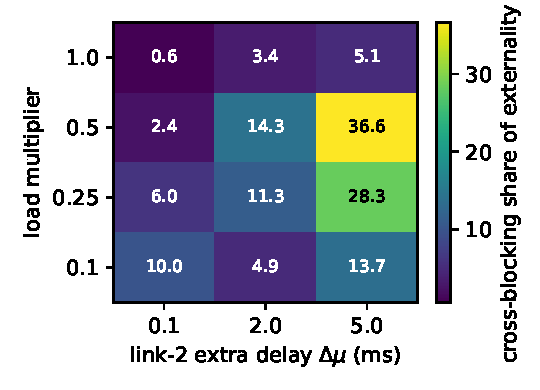
\includegraphics[width=0.5\linewidth]{fig_share.pdf}
\caption{Cross-blocking's share of the externality (\%) against load and asymmetry (\tagE{}).}
\end{figure}
Queueing/service delay accounts for \SBBNetMin{}--\SBBNetMax{} of the externality across cells, self-reordering for at most \SBBSelfAbs{} in absolute value, and cross-blocking for \SBBCrossMin{} (load \SBBMinCrossLoad{}, smallest asymmetry) up to \SBBCrossMax{} (load \SBBMaxCrossLoad{}, \SBBMaxCrossAsym{}~ms asymmetry), median \SBBCrossMed{}, below 15\% in \SBBCrossBelowFifteen{} cells. The share grows with link asymmetry. This also explains the V3 failure: at 25\% load with 2~ms asymmetry the share was well below the required 0.75.

\section{Study 3: boundary, replication and decision utility}\label{sec:s3}
\paragraph{H10 (preregistered): pinned disjoint links.} Proposition~\ref{prop:cond} predicts that when flows are pinned to different links the gap $|E-X|/E$ is near zero, while for flows sharing links it is not. Result (\tagC{}, 100 seeds): gap \TenGapPinned{} \TenGapPinnedCI{} for pinned flows against \TenGapShared{} \TenGapSharedCI{} for flows sharing both links, so H10 is supported. Pinning also shrinks the externality itself (mean \TenEPinned{}~ms against \TenESharedF{}~ms; descriptive). \textbf{A preregistered exact check, V7, failed:} the maximum per-run residual $|E-X|$ on clean runs was \TenVSeven{}~ms rather than at rounding level. A post hoc diagnosis, verified in the stored rows, is that one of 200 rows had different delivered-packet counts in the full and solo runs (a packet still held in the reorder buffer at the horizon); the other 199 rows agree to rounding error. We report V7 as failed with this diagnosis.
Exploratory X6 asked whether the pinned flows still interact through the shared sequence-number window. Dispatch stalls occurred in at most \SXSixMaxStall{} of runs, and the gap with a 64-entry window was \SXSixGapLow{} at nominal load and \SXSixGapHigh{} \SXSixGapHighCI{} at 1.4$\times$ load, where the externality is tiny (\SXSixEHigh{}~ms), so exactness holds only up to finite-horizon composition effects.

\paragraph{H11 (preregistered): ns-3 replication.} Study~2 suggested that trace-level cross-blocking is a small share of the externality. H11 asked whether this holds in ns-3: it was to be called replicated if cross-blocking was a small share (interval upper bound below 0.5) in at least two thirds of defined cells, and not replicated if at least a third of cells had a share of at least one half. With \ElevenRuns{} new runs without the bulk flow, the share ranged from \ElevenMin{} to \ElevenMax{} (\ElevenMostly{} of \ElevenDefined{} cells at or above one half, \ElevenLittle{} below), so \textbf{H11 is not replicated}: the share is regime dependent and the heavy-load figure of Study~2 must not be generalised.
\begin{table}[h]
\centering\small
% AUTO-GENERATED
\begin{tabular}{lrrr}
\toprule
ns-3 cell & $E$ (ms) & share $r$ & $r$ interval\\
\midrule
A0 / L0 & 0.019 & 87\% & [87\%, 88\%]\\
A0 / L1 & 0.102 & 4\% & [4\%, 4\%]\\
A0 / L2 & 0.328 & 9\% & [8\%, 9\%]\\
A1 / L0 & 0.022 & 80\% & [79\%, 82\%]\\
A1 / L1 & 0.123 & 24\% & [24\%, 25\%]\\
A1 / L2 & 0.400 & 16\% & [15\%, 16\%]\\
A2 / L0 & 0.133 & 88\% & [87\%, 89\%]\\
A2 / L1 & 0.255 & 64\% & [64\%, 65\%]\\
A2 / L2 & 0.611 & 40\% & [40\%, 41\%]\\
\bottomrule
\end{tabular}

\caption{Study 3, H11 (\tagC{}): externality of the bulk flow on the latency-sensitive flow and the share explained by trace-level cross-blocking, ns-3.47 FIFO, 30 seeds per arm. Intervals are bootstraps over seeds, arms resampled independently.}
\end{table}

\paragraph{H12 (preregistered, flawed) and X7 (exploratory): decision utility.} H12 asked whether choosing the flow to remove by Shapley blame beats choosing it by trace blame. The preregistered gain metric weighted victims by flow weight while excluding the removed flow, which penalises removing heavy flows; we found this misalignment \emph{after} seeing the results. The formal outcome (Shapley minus trace gain \TwelveFlawSASPDiff{}, \TwelveFlawSASPCI{} under FullSASP, reversed in sign under FIFO) is therefore not used as evidence. An aligned re-test on fresh seeds (X7, \tagE{}) found no difference under FullSASP (both policies pick the same flow) and \SXSevenFifoDiff{} \SXSevenFifoCI{} under FIFO. \textbf{We therefore claim no decision advantage for Shapley attribution.}

\section{Study 4: the single-trace certificate on held-out cells}\label{sec:s4}
Exploratory inspection of the 21 cells of Studies~2b and~3 (the training set) showed $r\ge q$ in all of them and a Spearman correlation of 0.85, and led to Proposition~\ref{prop:cert}. Study~4 was preregistered on \FourCells{} fresh cells and nothing was tuned on them: 13 Python cells (four or eight flows, load multipliers, link-2 delays) and 6 ns-3 cells (two conditions, three bulk fractions, \FourNsRuns{} runs with and without bulk). The tests were:
H13, $r\ge q$ in every defined Python cell (exact) and, counted, in ns-3 at the point estimate, also with the floor $d_{\min}=1.69$~ms for the Python simulator;
H14, pooled Spearman$(q,r)\ge0.70$ with a cell-bootstrap lower bound above 0.40;
H15 (descriptive), the cut-off $q\ge0.30$ frozen from the training set as a predictor of $r\ge0.5$.
All \FourDefined{} cells were defined (externality interval above zero), so none was excluded.
\begin{table}[h]
\centering\small
% AUTO-GENERATED
\begin{tabular}{lrrrc}
\toprule
held-out cell & $E$ (ms) & $r=X/E$ & $q=X/\mathrm{e2e}$ & $r\ge q$\\
\midrule
S4 $\lambda$=0.15 $\Delta\mu$=0.5 & 0.072 & 0.8\% & 0.0\% & yes\\
S4 $\lambda$=0.15 $\Delta\mu$=1.0 & 0.133 & 1.9\% & 0.1\% & yes\\
S4 $\lambda$=0.15 $\Delta\mu$=3.0 & 0.398 & 12.4\% & 2.1\% & yes\\
S4 $\lambda$=0.35 $\Delta\mu$=0.5 & 0.182 & 2.6\% & 0.2\% & yes\\
S4 $\lambda$=0.35 $\Delta\mu$=1.0 & 0.302 & 4.6\% & 0.6\% & yes\\
S4 $\lambda$=0.35 $\Delta\mu$=3.0 & 0.838 & 20.7\% & 5.9\% & yes\\
S4 $\lambda$=0.75 $\Delta\mu$=0.5 & 0.680 & 2.2\% & 0.6\% & yes\\
S4 $\lambda$=0.75 $\Delta\mu$=1.0 & 1.042 & 5.0\% & 1.7\% & yes\\
S4 $\lambda$=0.75 $\Delta\mu$=3.0 & 2.759 & 15.6\% & 8.2\% & yes\\
S8 $\lambda$=0.5 $\Delta\mu$=0.5 & 0.333 & 2.5\% & 0.4\% & yes\\
S8 $\lambda$=0.5 $\Delta\mu$=3.0 & 1.418 & 23.0\% & 9.4\% & yes\\
S8 $\lambda$=1.0 $\Delta\mu$=0.5 & 2.093 & 1.3\% & 0.7\% & yes\\
S8 $\lambda$=1.0 $\Delta\mu$=3.0 & 14.036 & 4.3\% & 3.7\% & yes\\
A1 F0.15 & 0.009 & 121.7\% & 9.7\% & yes\\
A1 F0.45 & 0.058 & 55.8\% & 20.4\% & yes\\
A1 F0.7 & 0.230 & 11.8\% & 8.2\% & yes\\
A2 F0.15 & 0.056 & 127.4\% & 34.9\% & yes\\
A2 F0.45 & 0.128 & 71.1\% & 33.0\% & yes\\
A2 F0.7 & 0.327 & 43.3\% & 29.9\% & yes\\
\bottomrule
\end{tabular}

\caption{Study 4 (\tagC{}): held-out cells. Python cells: four-flow (S4) or eight-flow (S8) system, load multiplier $\lambda$ and link-2 extra delay; ratios of sums over 100 seeds and all victims. ns-3 cells: condition and bulk fraction of capacity, ratios of means over 30 seeds per arm.}\label{tab:s4}
\end{table}
\begin{figure}[h]
\centering
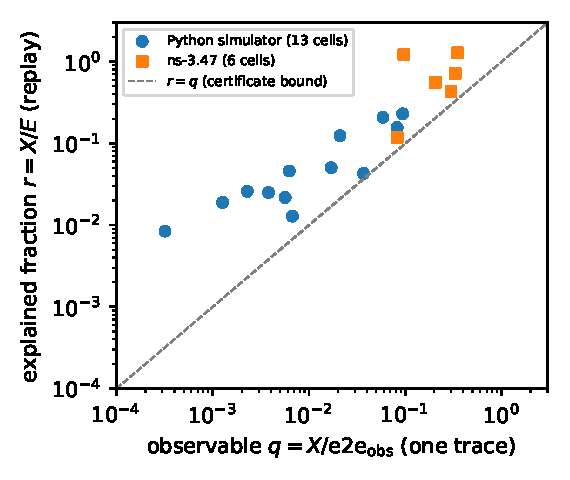
\includegraphics[width=0.55\linewidth]{fig_cert.pdf}
\caption{Study 4 (\tagC{}): observable share $q$ against explained fraction $r$ for the held-out cells; every point lies on or above the dashed line $r=q$.}
\end{figure}
\paragraph{Results.} H13 \textbf{confirmed}: \FourPyViol{} violations in the Python cells (also \FourPyFloorViol{} with the $d_{\min}$ floor), \FourNsViol{} in the ns-3 cells at the point estimate. H14 \textbf{confirmed}: pooled $\rho=\FourRho$ (\FourRhoCI{}). H15: precision \FourPrec{} and recall \FourRecall{} (\FourTP{} true positives, \FourFP{} false positives, \FourFN{} false negatives; only four positives, so descriptive).
\paragraph{How to read this honestly.} (i) The pooled correlation is helped by the two platforms occupying different ranges: Python cells have $q$ of \FourPyQMin{}--\FourPyQMax{} and $r$ of \FourPyRMin{}--\FourPyRMax{}, ns-3 cells $q$ of \FourNsQMin{}--\FourNsQMax{} and $r$ of \FourNsRMin{}--\FourNsRMax{}; within platform the correlations are \FourRhoPy{} (13 cells) and \FourRhoNs{} (6 cells, no interval preregistered). (ii) The bound is loose when $q$ is small: the median ratio $r/q$ is \FourRatioMedPy{} in the Python cells (maximum \FourRatioMaxPy{}) and \FourRatioMedNs{} in the ns-3 cells. An exploratory linear fit of $r$ on $q$ has slope \FourOLSSlope{} and $R^2=\FourOLSRsq$; $q$ is a guarantee and a ranking, not an estimate. (iii) In \FourNsRAboveOne{} ns-3 cells $r>1$: the mean cross-wait exceeds the unpaired-noise estimate of the externality when that externality is only \FourNsEOverMin{}--\FourNsEOverMax{}~ms, so $r$ is not a bounded fraction under estimation noise (the certificate $r\ge q$ is unaffected).
\paragraph{Validity.} V10 passed: \FourVTenSig{} replay-signature violations in \FourVTenRows{} rows and an identity gap of at most \FourVTenGap{} (the preregistered 5\% sample and all rows). V11 passed: every without-bulk ns-3 run sent no bulk packets and had zero cross-wait, and the runtime audit counters were clean. A first analysis run flagged the two ARP priming frames present in every run (also in all earlier campaigns) as a violation because the check was stricter than the frozen audit rule (at most 20 untagged frames); we corrected the check to the frozen rule, which did not change any hypothesis outcome.

\section{Simulator and evaluation audit (Study 1)}\label{sec:audit}
Study 1 preregistered six hypotheses about implicit invariants, with exact oracles and controls, on seeds 7000--7099.
\begin{table}[h]
\centering\small
\begin{tabular}{p{0.06\linewidth}p{0.52\linewidth}p{0.3\linewidth}}
\toprule
 & Primary measure & Outcome \\
\midrule
H1 & shared-stream arrival mismatches \OneMismatchShared{}; $\Delta\rho=\DeltaRhoTwo$ \DeltaRhoTwoCI{} & \HOneVerdictTwo{} \\
H2 & undelivered fraction \UndelFracFIFO{} (threshold \UndelThreshold) & \HTwoVerdict{} \\
H3 & paired-CI width ratio keyed/shared \WidthRatioTwo{} & \HThreeVerdictTwo{} \\
H4 & $|\Delta S_1|/S_1=\HFourRatioFIFO$ \HFourRatioFIFOCI{}; trace control \HFourTrace{} & violation \HFourVerdict{} \\
H5 & loss draws/attempt $\neq1$ in \OFiveRate{}; burst length \BurstShipped{} vs.\ \BurstSingle{} & \HFiveVerdict{} \\
H6 & violating seeds FIFO \HSixFIFO{}, FullSASP \HSixFullSASP{}, MeanOnly \HSixMeanOnly{}; leak control \HSixLeakyGlobal{} & \HSixVerdict{} \\
\bottomrule
\end{tabular}
\caption{Study 1 preregistered outcomes (\tagC{}).}
\end{table}
The shared random stream did not desynchronise arrivals; keyed noise did not tighten paired intervals (width ratio \WidthRatioTwo{}); survivor bias was immaterial. Three consequences matter here. First, \textbf{H4}: self-blocking is invariant on a fixed trace but changed by \HFourRatioFIFO{} (about \HFourUnits{}~$\mu$s) when the competitor was removed from the system, the observation that motivated the externality concept. Second, \textbf{H5}: every attempt drew two loss variables (\OFiveRate{}), shortening burst length by \BurstRelAbs{}; in an exploratory run absolute weighted blocking under bursts changed from \XTwoMShipFIFO{} to \XTwoMSingleFIFO{} while the FIFO-to-FullSASP reduction stayed near \XTwoRedShip{} (shipped) against \XTwoRedSingle{}. Third, \textbf{effect sizes}: the scheduler's gain in $M$ from 1000 fresh seeds is \XFourDShared{} (\XFourCIShared{}) against \OldD{} (\OldDCI{}) from the earlier 30-seed campaign, \OldRatio{}$\times$ larger but with overlapping intervals (\tagE{}, \tagP{}). Pairing between arms weakens with link asymmetry under both shared and keyed streams (Figure~\ref{fig:pair}, \tagE{}) and varies from \XFiveRhoMin{} to \XFiveRhoMax{} across pre-existing ns-3 cells while offered traffic was identical in \XFiveIdentical{} of \XFiveTriples{} triples, so weak pairing reflects scheduler-induced divergence, not random-number design. The causality check passed for all real schedulers but, at release level, could not see a one-millisecond look-ahead (\HSixLeakyLocal{}); a decision-level comparison caught it in \XThreeLeakyLocal{} (\tagE{}).
\begin{figure}[h]
\centering
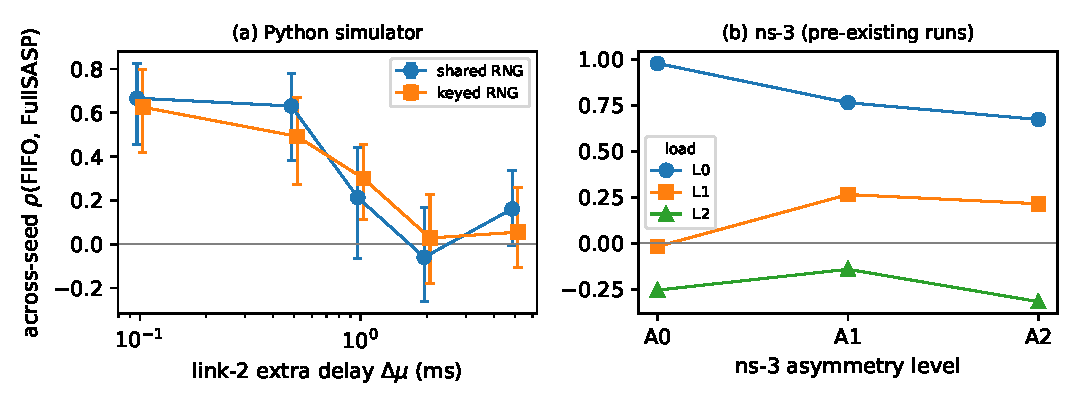
\includegraphics[width=0.9\linewidth]{fig_pairing.pdf}
\caption{Across-seed correlation between FIFO and FullSASP (\tagE{}; panel b: \tagP{}).}\label{fig:pair}
\end{figure}

\section{Claim-to-evidence table}
Tags: \tagC{} preregistered confirmatory; \tagE{} exploratory; \tagP{} analysis of pre-existing data; \tagA{} analytic.
\begin{table}[h]
\centering\footnotesize
\begin{tabular}{p{0.30\linewidth}p{0.27\linewidth}p{0.15\linewidth}p{0.2\linewidth}}
\toprule
Claim & Evidence & Tag & Result file \\
\midrule
Externality splits exactly into queueing, self, cross parts & identity gap \SBBIdentity{}; held-out \FourVTenGap & \tagA{}, \tagE{}, \tagC{} & exploratory\_study2b, analysis\_study4 \\
Shapley blame is efficient & gap \SBVone & \tagA{}, \tagC{} & analysis\_study2 \\
Certificate $r\ge q$ holds & \FourPyViol{} Python, \FourNsViol{} ns-3 violations & \tagA{}, \tagC{} & analysis\_study4 \\
$q$ ranks cells by $r$ & $\rho=\FourRho$ \FourRhoCI & \tagC & analysis\_study4 \\
Cut-off $q\ge0.30$ finds $r\ge0.5$ & precision \FourPrec, recall \FourRecall & descriptive & analysis\_study4 \\
Pinned disjoint links: trace $\approx$ intervention & gap \TenGapPinned{} vs.\ \TenGapShared & \tagC (V7 failed) & analysis\_study3\_python \\
Cross-blocking share is regime dependent & ns-3 \ElevenMin{}--\ElevenMax; Python \SBBCrossMin{}--\SBBCrossMax & \tagC{}, \tagE{} & analysis\_study3\_ns3, exploratory\_study2b \\
Small share at heavy load (Python only) & \SBrFour{} \SBrFourCI & \tagC (V3 failed) & analysis\_study2 \\
Trace blame misranks flows & $\tau=\SBtauFour$ \SBtauFourCI & \tagC (V3 failed) & analysis\_study2 \\
Externalities are non-additive & $R=\SBRFour$ \SBRFourCI & \tagC & analysis\_study2 \\
Shapley guides removal better than trace blame & not supported (X7) & \tagE & exploratory\_study3 \\
Self-blocking invariant only on a trace & \HFourRatioFIFO{}; control \HFourTrace & \tagC & analysis \\
Two loss draws per attempt & \OFiveRate{} & \tagC & analysis \\
Gain estimate shrinks with more seeds & \OldD{} vs.\ \XFourDShared & \tagE{}, \tagP{} & exploratory \\
\bottomrule
\end{tabular}
\caption{Every number resolves to a stored result file through \texttt{make\_numbers.py}.}
\end{table}

\section{Discussion}
\paragraph{What a practitioner can do with this.} Given a single simulation trace, compute $q$. If $q$ is large, the certificate guarantees that trace-level cross-blocking is at least that share of the externality, so the trace figure is a defensible summary; in our data this happened in a minority of cells (Table~\ref{tab:s4}). If $q$ is small, the trace figure may badly understate the harm one flow does another (the Python cells show $r$ up to \FourPyRMax{} while $q$ stays below \FourPyQMax{}), and a counterfactual replay is needed. Replay requires noise keyed per flow and packet so that removing a flow leaves the others' draws unchanged; this is cheap in a simulator.
\paragraph{Why the headline changed.} Study~2 reported that cross-blocking is a small share of the externality. That is true at its heavy-load operating point in the Python simulator and false in several ns-3 conditions. The defensible statement is regime dependence plus a way to bound it from a trace, and the paper is framed that way.
\paragraph{Design implication, not tested.} Pinning flows to disjoint links makes the two notions coincide (Proposition~\ref{prop:cond}) and shrinks the externality here, at the cost of load balancing; quantifying that trade-off, and whether scheduling by externality pays off, is future work and is not claimed.

\section{Limitations}
\begin{itemize}
  \item \textbf{Simulation only.} A purpose-built Python simulator and a patched ns-3.47 build, two links, short horizons, one latency-sensitive and one bulk flow in ns-3. The ns-3 binary carries this project's modifications, so it is a second implementation, not an independent one. No hardware or trace data.
  \item \textbf{The Study 2 validity control failed} (V3), so H7--H9 are not independently validated; the replacement evidence (identity, sweep) is exploratory.
  \item \textbf{The H10 exact check V7 failed} with a verified single-row diagnosis; the H12 design was flawed and its formal outcome is not used.
  \item \textbf{The certificate is one-sided and loose for small $q$} (median $r/q$ \FourRatioMedPy{} in Python). The ranking evidence is pooled across two platforms (within-platform \FourRhoPy{} and \FourRhoNs{}, the latter on six cells), the cut-off has only four positive cells, and the certificate was discovered on a training set examined after the fact (21 cells; disclosed in the preregistration) before being tested on 19 fresh cells.
  \item \textbf{The ns-3 ``$X$'' is the binary's cross-wait column}, which charges the whole wait to a cross-flow binding blocker and so includes the self-blocking part of those packets. A later check (Study~6, conditions A1 and A2, loads L0--L2, 60 runs) found the pure cross-blocking to be at least 98.8\% of it in every cell (99.5\% overall); condition A0 was not measured.
  \item \textbf{ns-3 externality is an unpaired difference}, noisy when small; $r>1$ occurs in \FourNsRAboveOne{} cells. The guarantee is tested at the point estimate only.
  \item Under FIFO the flows are nearly exchangeable, so the ranking test H8 has little signal; the unequal-flow evidence (SASP) is exploratory.
  \item The Shapley value is one attribution; with strongly convex externalities ($R=\SBRFour$) other allocations answer different questions. No allocation comparison was made beyond X7.
  \item Means are over delivered packets in Studies 2b--4; Study 2 uses right-censored means. Censoring was negligible at these horizons but was not varied.
  \item The audit's pilot seeds 1--40 were examined before an amendment (disclosed in the preregistration); confirmatory seeds were untouched. The seed of the 5\% identity sample in V10 was fixed by the analysis script, not by the preregistration.
  \item The literature search was limited; unverifiable inherited references were excluded. $p$-values (Study 1) use a sign-flip test; no human annotation, model judge or hardware measurement was used.
\end{itemize}

\section{Conclusion}
A receiver trace tells a designer what a packet waited for, not what the system would have done without the other flow. We make the difference exact (an accounting identity, a boundary condition, and a one-sided certificate computable from a single trace), show that the trace figure is faithful in some regimes and a poor proxy in others, and report the failed control, the failed exact check and the flawed decision test that bound the claims. Whether externality-aware scheduling pays off remains open.

\section*{Reproducibility}\label{sec:repro}
All materials are in \texttt{validation/pairing/}. Study 1: preregistration \texttt{d3b1131} (SHA-256 \texttt{abf0c16a\dots}), Amendment~1 \texttt{d7eeda6}, Amendment~2 and harness \texttt{f44b970}, results \texttt{3000f3f}. Study 2: preregistration \texttt{477a64a} (\texttt{73c53be0\dots}); results and Study 2b plan \texttt{cce5dce}. Study 3: preregistration \texttt{646c974} (\texttt{0cc9b333\dots}), amendment and exploratory plan with Python results \texttt{6073e71} (\texttt{9198268\dots}), ns-3 results \texttt{ba6eff7}, exploratory X6/X7 \texttt{b7675c0}. Study 4: preregistration \texttt{b7675c0} (\texttt{15e5dd54\dots}), results \texttt{cbde577}. Raw-file hashes: \texttt{results/RAW\_AND\_ANALYSIS.sha256}, \texttt{STUDY2\_RAW.sha256}, \texttt{STUDY3\_PY\_RAW.sha256}, \texttt{STUDY3\_NS3\_RAW.sha256}, \texttt{STUDY4\_RAW.sha256}. Rebuild with the \texttt{run\_study*.py} and \texttt{analyze*.py} scripts, then \texttt{paper/make\_numbers.py} and \texttt{paper/make\_fig.py}. Decisions are logged in \texttt{decisions.md}.

\bibliographystyle{plain}
\bibliography{refs}
\end{document}
